\documentclass[spanish, DIV=calc, paper=a4, fontsize=11pt, twocolumn]{scrartcl}	 % A4 paper and 11pt font size

\usepackage[utf8x]{inputenc}
\usepackage{lipsum} % Used for inserting dummy 'Lorem ipsum' text into the template
\usepackage[spanish]{babel} % English language/hyphenation
\usepackage[protrusion=true,expansion=true]{microtype} % Better typography
\usepackage{amsmath,amsfonts,amsthm} % Math packages
\usepackage[svgnames]{xcolor} % Enabling colors by their 'svgnames'
\usepackage[hang, small,labelfont=bf,up,textfont=it,up]{caption} % Custom captions under/above floats in tables or figures
\usepackage{booktabs} % Horizontal rules in tables
\usepackage{fix-cm}	 % Custom font sizes - used for the initial letter in the document

\usepackage{sectsty} % Enables custom section titles
\allsectionsfont{\usefont{OT1}{phv}{b}{n}} % Change the font of all section commands

\usepackage{fancyhdr} % Needed to define custom headers/footers
\pagestyle{fancy} % Enables the custom headers/footers
\usepackage{lastpage} % Used to determine the number of pages in the document (for "Page X of Total")

% Headers - all currently empty
\lhead{}
\chead{}
\rhead{}

% Footers
\lfoot{}
\cfoot{}
\rfoot{\footnotesize Page \thepage\ of \pageref{LastPage}} % "Page 1 of 2"

\renewcommand{\headrulewidth}{0.0pt} % No header rule
\renewcommand{\footrulewidth}{0.4pt} % Thin footer rule

\usepackage{lettrine} % Package to accentuate the first letter of the text
\newcommand{\initial}[1]{ % Defines the command and style for the first letter
\lettrine[lines=3,lhang=0.3,nindent=0em]{
\color{DarkGoldenrod}
{\textsf{#1}}}{}}

% Background - background image
\usepackage{graphicx}
\usepackage{eso-pic}
\newcommand\BackgroundPic{
\put(-5,105){
\parbox[b][\paperheight]{\paperwidth}{%
%\vfill
\centering

\includegraphics[width=\paperwidth,height=\paperheight,
keepaspectratio]{img/background.png}%
\vfill
}}}

%----------------------------------------------------------------------------------------
%	TITLE SECTION
%----------------------------------------------------------------------------------------

\usepackage{titling} % Allows custom title configuration

\newcommand{\HorRule}{\color{DarkGoldenrod} \rule{\linewidth}{1pt}} % Defines the gold horizontal rule around the title

\pretitle{\vspace{-30pt} \begin{flushleft} \HorRule \fontsize{40}{40} \usefont{OT1}{phv}{b}{n} \color{DarkRed} \selectfont} % Horizontal rule before the title

\title{dondeEstaciono} % titulo del proyecto

\posttitle{\par\end{flushleft}\vskip 0.5em} % Whitespace under the title

\preauthor{\begin{flushleft}\large \lineskip 0.5em \usefont{OT1}{phv}{b}{sl} \color{DarkRed}} % Author font configuration

\author{Nicolás Alderete, Germán Romero, Joel del Valle} % Your name

\postauthor{\footnotesize \usefont{OT1}{phv}{m}{sl} \color{Black} % Configuration for the institution name
\newline{Tecso -- Equipo Integración en el Cliente: Interbanking} % Your institution

\par\end{flushleft}\HorRule} % Horizontal rule after the title

\date{\today\\v1.7}

%----------------------------------------------------------------------------------------

\begin{document}

\AddToShipoutPicture*{\BackgroundPic}

\maketitle % Print the title

\thispagestyle{fancy} % Enabling the custom headers/footers for the first page 



%----------------------------------------------------------------------------------------
%	BREVE DESCRIPCION DEL PROYECTO
%----------------------------------------------------------------------------------------

\initial{E}\textbf{l presente documento tiene como objetivo acercar una propuesta para el desarrollo de una aplicación 
centrada en la gestión de estacionamientos y uso de los mismos, ésta se compone de una app mobile para los clientes
de estacionamientos (a los que llamaremos US), una app mobile y una app web para los estacionamientos (a los que llamaremos EST). También la app web contendrá las funcionalidades presentes en la versión mobile de los US fuera del perfil de los EST.
Esta propuesta pretende generar un proyecto que ayude a posicionar mejor a Tecso en el mundo de aplicaciones mobile. Generado, a partir de éste proyecto de innovación, tanto en tecnologías como en servicios a brindar.}

%----------------------------------------------------------------------------------------
%	DESCRIPCION DE LAS APP MOBILE Y WEB:
%----------------------------------------------------------------------------------------

\section{Descripción}

\subsection{AppMobile para US}
Tendríamos dos versiones, una gratis y una paga.

Cada vez que el US se encuentre en la visión Mapa, éste podrá ver todos los EST registrados y toda la información disponible cerca a su posición. En caso de haber Marketing en Real Time (RTM) también se visualizaría.

\begin{enumerate}

	\item versión gratis, funcionalidades:
		
		\begin{enumerate}
			
			\item donde estoy?: indica en un mapa la posición del celular

			\item información estática de los estacionamientos registrados (donde queda, cantidad de lugares totales, horarios y precios)

			\item función gps para indicar como llegar a los estacionamientos registrados

			\item funcionalidad para calificar ó denunciar a un estacionamiento

		\end{enumerate}

	\item versión paga, funcionalidades:

		\begin{enumerate}
			
			\item información de los estacionamientos (donde queda, horarios, precios, disponibilidad de lugares en tiempo real, tiempo de demora en tiempo real)

			\item donde estoy?: indica en un mapa la posición del celular

			\item función gps para indicar como llegar a los estacionamientos registrados

			\item donde me estacione?: indica un punto en el mapa donde se dejo el auto

			\item como llegar a mi auto?: función gps que muestre como llegar al punto donde se estacionó el auto
					
			\item reservar lugar: función de reservar lugares en estacionamientos, siempre que estos tengan habilitado el servicio (esto es un servicio pago para los EST)

			\item marketing: función que lista promociones o publicidades de los estacionamientos, se podrá filtrar por zonas o lugares específicos (esto es un servicio pago para los EST)

			\item marketing-real-time: función que muestra las promociones o publicidades en el mapa en tiempo real cuando se utiliza el gps (esto es un servicio pago para los EST). Esta funcionalidad podría extenderse a otros rubros que no sean los EST\footnote[1]{"Fede Repond nos comento sobre el proyecto Nextoo, y creemos que podemos enlazarlo con esta funcionalidad o bien utilizar el conocimiento adquirido en ese desarrollo"}

			\item función favoritos: guardar puntos en el mapa que el usuario desee

			\item funcionalidad para calificar ó denunciar a un estacionamiento

		\end{enumerate}

\end{enumerate}

\subsection{AppWeb para US}
Dentro de la misma AppWeb para EST pero sin necesidad de un login, los usuarios podrán utilizar las siguientes funcionalidades:

\begin{enumerate}
	
	\item visualizar todos los EST y su información (donde queda, horarios, precios, disponibilidad de lugares en tiempo real, tiempo de demora en tiempo real, y que servicios tiene contratado), ya sea en un listado o en el mapa.

	\item funcionalidad de como llegar a los EST

\end{enumerate}

\subsection{AppWeb para EST}
Dependiendo del servicio que contrate el EST deben mostrarse diferentes funcionalidades. La contratación es gratis y solo cobraríamos por servicios adicionales	

\begin{enumerate}
	
	\item la contratación gratis incluye:

		\begin{enumerate}
		
			\item posibilidad de cargar la información del EST, nombre, teléfono, email, cantidad de lugares totales, precios y horarios

			\item posibilidad de actualizar en tiempo real la disponibilidad de lugares

			\item ver estadísticas de cantidad de autos diarios, mensuales, etc.., y cuales son los horarios picos

		\end{enumerate}

	\item los servicios adicionales serían:

		\begin{enumerate}
			
			\item reserva online por parte de los US: los US, mediante la app mobile podrán reservar un lugar en el estacionamiento que deseen

			\item conectar el servicio de tickets que actualmente tenga un EST con la app web para que actualize automáticamente los lugares disponibles

			\item servicio de tickets (como el que existe actualmente) y que se enlace automáticamente con la disponibilidad de lugares

			\item servicio de tesorería, para el control del dinero

			\item marketing: posibilidad de crear ofertas o publicaciones por un tiempo determinado

			\item marketing-real-time: posibilidad de crear ofertas que se visualizaran en el gps de los US

		\end{enumerate}

\end{enumerate}

\subsection{AppMobile para EST}
Tendría las mismas funcionalidades gratis y servicios adicionales que la AppWeb para EST, solamente que mobile. Esto esta orientado a aquellos estacionamientos que no cuenten con una pc con conexión a internet y si con un celular con red de datos.

El único servicio que quedaría sin efecto, por ahora, sería el de servcio de tickets en caso de necesitar imprimir tickets fiscales

\section{Funcionamiento}

\subsection{AppMobile para US gratis}
Los US, al entrar a la app visualizaran varias opciones de acción, la primera indicará la funcionalidad "donde estoy?", al accionarla mostrará un mapa con la ubicación actual del celular (en el mapa, el US podra visualizar los EST que estan registrados). La segunda mostrará un listado de los EST registrados, estos estarán ubicados por zonas, asi que  también tendrá un filtro para poder realizar una busqueda mas acotada; desde esta pantalla al hacer click sobre cualquier estacionamiento se mostrará al EST en un mapa y se visualizará la información del estacionamiento, también contará con un botón que le permita utilizar la función gps para poder llegar al EST seleccionado. La última acción sera utilizada para que un US pueda calificar o denunciar un EST.
				
Cuando el US se encuentre utilizando la función gps en el mapa se visualizaran los EST registrados y la información de los mismos, pudiendo	cambiar de destino en cualquier momento

\subsection{AppMobile para US paga}
Los US, al entrar a la app tendrán varias opciones de acción. La primera, indicará la funcionalidad "donde estoy?", al accionarla mostrará un mapa con la ubicación actual del celular (en el mapa, el US podra visualizar los EST que estan registrados). 

La segunda mostrará un listado de los EST registrados, estos estarán ubicados por zonas, asi que también tendrá un filtro para poder realizar una busqueda mas acotada; desde esta pantalla al hacer click sobre cualquier estacionamiento se mostrará al EST en un mapa y se visualizará la información del estacionamiento mostrando la cantidad de lugares disponibles en tiempo real, también contará con un botón que le permita utilizar la función	gps para poder llegar al EST seleccionado.

La tercera tendrá la funcionalidad de favoritos, donde el usuario podrá guardar los EST que desee para acceder a ellos mas rápido, aca	también se mostrará la información del EST en tiempo real.
				
La cuarta, tendrá la funcionalidad de "donde me estacioné" permitiendo al sistema guardar la posición donde se estacionó el vehículo y marcando el camino para llegar a él. 	

La quinta, da la funcionalidad de reservar un lugar en un estacionamiento para un día y horario determinado. Se mostrará un listado de los EST que tengan el servicio de reservas (adicional) contradado, una vez que se seleccione el EST se enviará un pedido de reserva a éste, cuando el EST responda la solucitud de pedido de reserva el US recibira una notificación. Esta reserva será válida para el dia y hora seleccionado	por el US con una tolerancia máxima de 15 minutos. Asi mismo, esta reserva podría cancelarce utilizando el mismo medio de comunicación.

La sexta, mostrará un listado de publicidades u ofertas que los EST realicen.

La última acción sera utilizada para que un US pueda calificar o denunciar un EST.

Cuando el US se encuentre utilizando la función gps en el mapa se visualizaran los EST registrados, la información de los mismos en tiempo real y las publicidades u ofertas en tiempo real, pudiendo cambiar de destino en cualquier momento.

\subsection{AppWeb para EST sin servicios adicionales}
Los EST que esten registrados tendrán acceso a una web donde se podrán logear y accederán a su perfil, dentro de su perfil tendran tres (3) pantallas.


La primer pantalla mostrará la información del EST (nombre, dirección,  teléfono, email, cantidad de lugares totales, precios y horarios), esta información puede ser editada exceptuando la dirección. La dirección solo podría ser modificada por nosotros.	La segunda contendrá la forma de aumentar o disminuir la cantidad de lugares disponibles. Y la tercera contendrá las estadisticas.

También tendrá una pantalla para poder crear varios usuarios, o varios administradores.


\subsection{AppWeb para EST - Servicios Adicionales}

\begin{description}
	
	\item[Reservas Online] El EST recibirá una notificación de solicitud de pedido de reserva para un día y hora determinado (tendrá un tiempo de vida), ésta puede ser aprobada o rechazada, al ser aprobada se envía al US una notificación de aprobación que exipira 15 minutos pasada la hora establecida en la reserva.

Nueva funcionalidad dentro del perfil. 

	\item[Actualización de lugares disponibles mediante vinculación] Se vincularía cualquier sistema de tickets (control del tiempo de los vehículos) con la actualización de los lugares disponibles

	\item[Módulo de Control de Tiempo de los Vehículos]	Permite anotar el ingreso de un vehículo y calcular el tiempo dentro del EST. Se vincularía con las maquinas fiscales para la impresión de un ticket fiscal o generar un ticket provisorio. Esto se vincularia con los precios y horarios ya cargados y con las reservas.

Nueva funcionalidad dentro del perfil. 

	\item[Módulo Tesorería]	Funcionalidad para gestionar los ingresos y egresos de dinero. Estadísticas diarias y mensuales. Esto se vincularía con los precios, horarios, y con el módulo de control del tiempo de los vehículos.

Nueva funcionalidad dentro del perfil.
	
	\item[Marketing] Funcionalidad para crear ofertas o publicaciones por un periodo de tiempo determinado, o para una cantidad de US determninado

Nueva funcionalidad dentro del perfil.

	\item[Marketing-real-time] Funcionalidad que permite que se vean ofertas y publicidades cuando el US esta utillizando el gps y dentro de la pantalla se visualiza el EST (se mostrará algún indicador que determine que el EST tiene ofertas).

Nueva opción dentro de la funcionalidad de Marketing.

\end{description}

\subsection{AppMobile para EST}
Tendría las mismas funcionalidades gratis y servicios adicionales que la AppWeb para EST, solamente que mobile. Esto esta orientado a aquellos estacionamientos que no cuenten con una pc con conexión a internet y si con un celular con red de datos.

El único servicio que quedaría sin efecto, por ahora, sería el de servcio de tickets en caso de necesitar imprimir tickets fiscales


\begin{figure*}[htp]
\section{MockUp's}
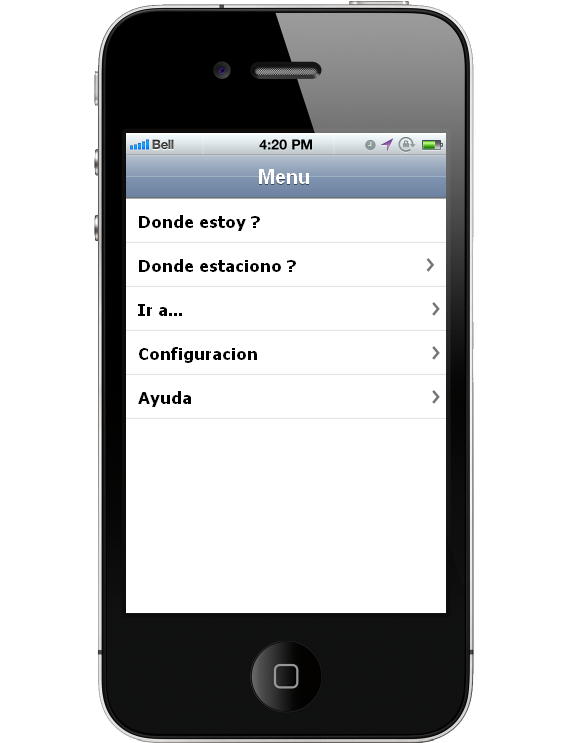
\includegraphics[width=8.0cm,height=\paperheight,keepaspectratio]{img/mockUpAppMobileUS/home.png}%
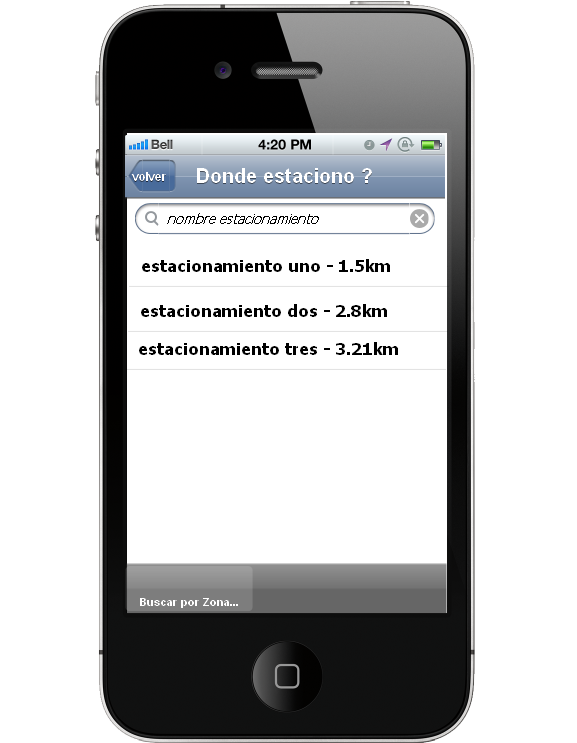
\includegraphics[width=8.0cm,height=\paperheight,keepaspectratio]{img/mockUpAppMobileUS/donde_estaciono_.png}%
\caption{MockUp AppMobile para US}
\label{dash-1}
\end{figure*}

\begin{figure*}[htp]
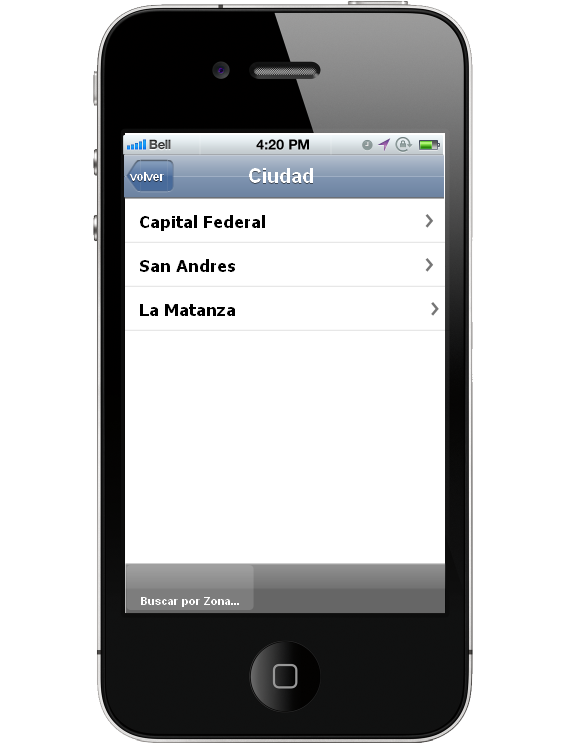
\includegraphics[width=8.0cm,height=\paperheight,keepaspectratio]{img/mockUpAppMobileUS/buscar1.png}%
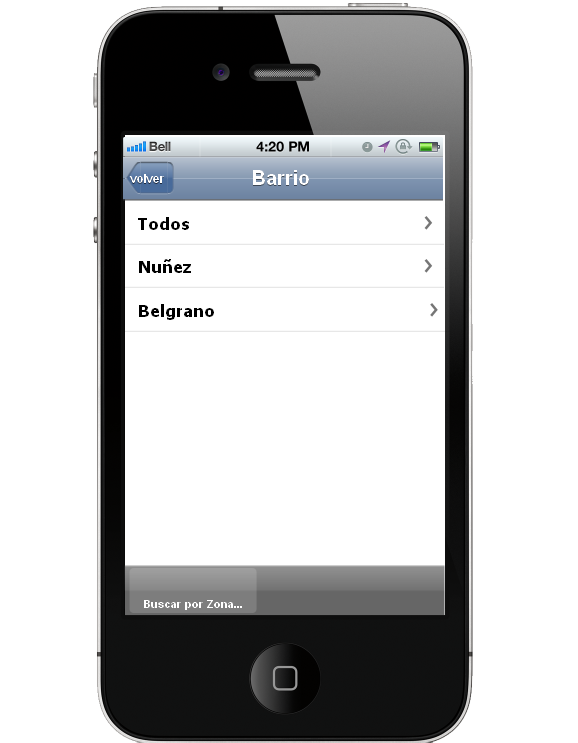
\includegraphics[width=8.0cm,height=\paperheight,keepaspectratio]{img/mockUpAppMobileUS/buscar2.png}%
\caption{MockUp AppMobile para US}
\label{dash-1}
\end{figure*}

\begin{figure*}[htp]
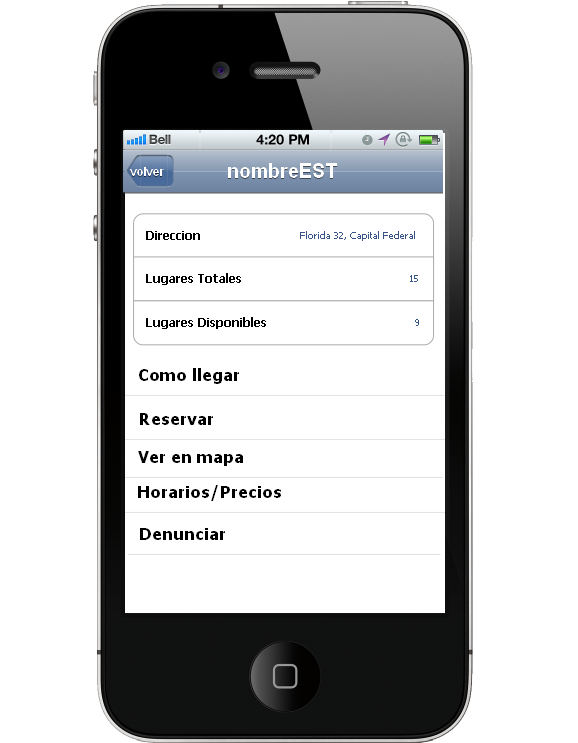
\includegraphics[width=8.0cm,height=\paperheight,keepaspectratio]{img/mockUpAppMobileUS/nombreestacionamiento.png}%
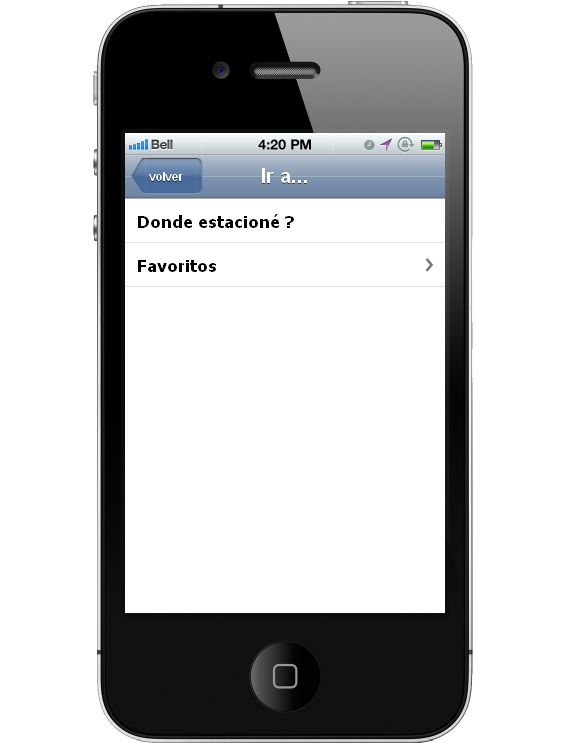
\includegraphics[width=8.0cm,height=\paperheight,keepaspectratio]{img/mockUpAppMobileUS/ira.png}%
\caption{MockUp AppMobile para US}
\label{dash-1}
\end{figure*}


\begin{figure*}[htp]
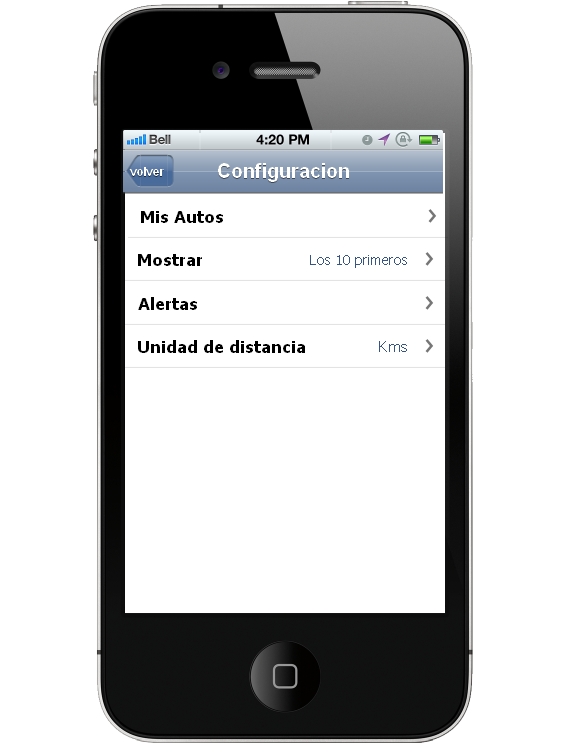
\includegraphics[width=8.0cm,height=\paperheight,keepaspectratio]{img/mockUpAppMobileUS/configuracion.png}%
\caption{MockUp AppMobile para US}
\label{dash-1}
\end{figure*}


\begin{figure*}[htp]
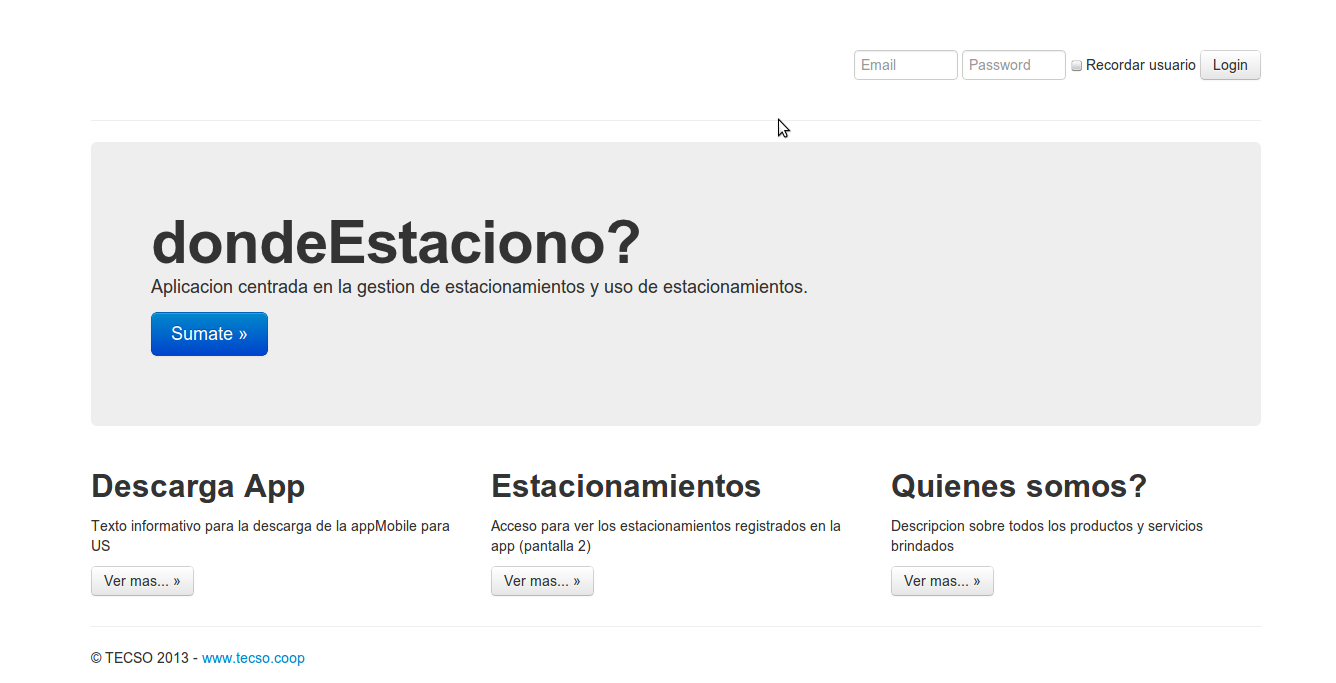
\includegraphics[width=18.0cm,height=\paperheight,keepaspectratio]{img/mockUpAppWeb/appWeb-01-01.png}%
\caption{MockUp AppWeb}
\label{dash-1}
\end{figure*}


\begin{figure*}[htp]
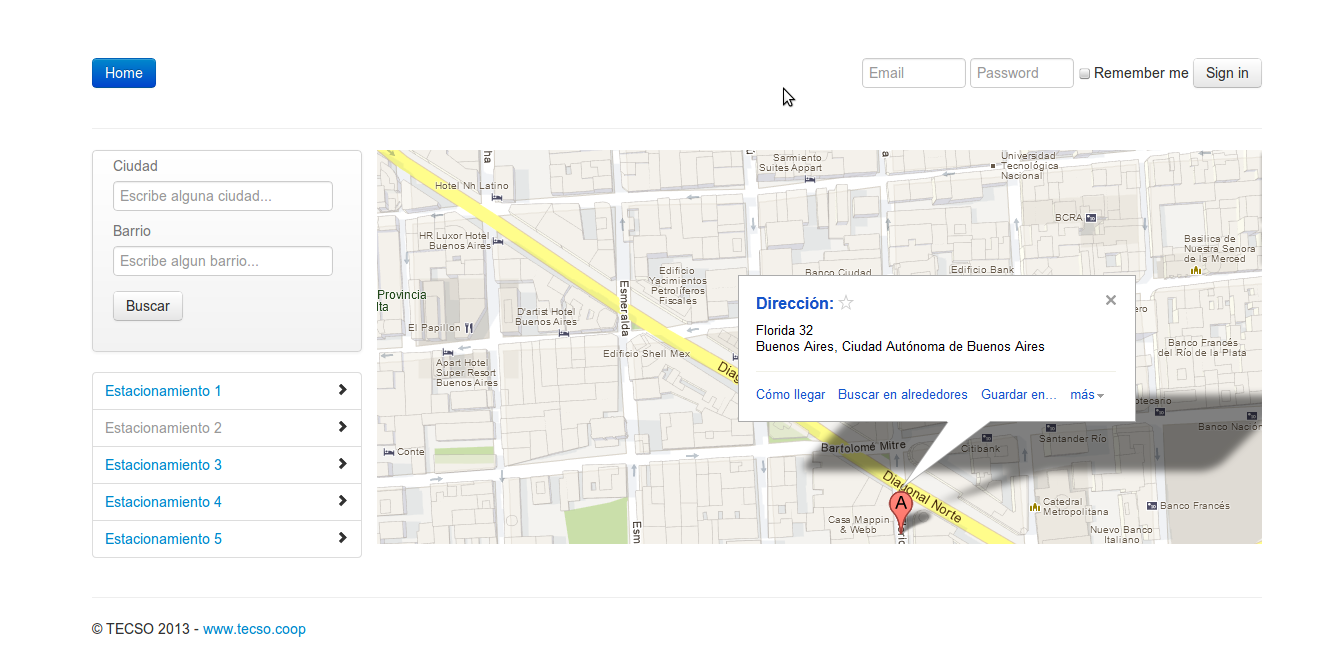
\includegraphics[width=18.0cm,height=\paperheight,keepaspectratio]{img/mockUpAppWeb/appWeb-02-02.png}%
\caption{MockUp AppWeb}
\label{dash-1}
\end{figure*}


\section{Tecnologías}
Como estamos dentro del proyecto tecsoIdeas, donde fomentamos la innovación, que mejor que utilizar algunas tecnologías que habitualmente no usamos, no?
	
	\begin{itemize}

		\item Para la app web
				
			\begin{itemize}
				\item[-] python 2.7
				\item[-] flask 0.9 + twitter boostrap
				\item[-] restful para conectarnos al server
			\end{itemize}			
					  
		\item Para la app mobile
				
			\begin{itemize}
				\item[-] java 1.6
				\item[-] phonegap
				\item[-] restful para conectarnos al server
				\item[-] hsqldb interna
			\end{itemize}

		\item Para el server
			\begin{itemize}
				\item[-] java 1.6
				\item[-] restful como webService
				\item[-] spring
				\item[-] mongoDB
			\end{itemize}

	\end{itemize}


\section{Próximos Pasos}
Si éste proyecto recibe el OK, tendríamos que empezar a armar un Proyecto, dando tiempos y prioridades de desarrollo. Al mismo tiempo deberiamos armar un plan de negocio para ofrecer este nuevo servicio.

Debido a que nosotros (ger, nico y joe) estamos en un cliente estaría bueno poder contar con 1 o 2 días mensuales para dedicarle tiempo completo al desarrollo del proyecto, esto significaría ir a trabajar a las oficinas de tecso y para eso necesitamos gestionar estos dias con Interbanking. 
				
También necesitariamos lugar en el svn y si todo camina poder tener un servidor (o un pedacito de uno) que soporte java y python.

\end{document}
